\section{Выводы} \label{economics_conclusion}

Результаты проведённых организационно-экономических расчетов позволили оценить структуру работ, необходимое количество исполнителей, структуру затрат проекта, срок окупаемости проекта.

\begin{enumerate}
	\item Общие затраты труда для выполнения программного проекта составили 77 чел/дней или 616 чел/часов. Затраты на разработку ПО составляют 545871,29 рублей.
	\item Исходя из временных требований к реализации проекта, была определена численность исполнителей: 2 человека. По результатам построения сетевого графика и диаграммы Гантта можно сделать вывод о том, что введение дополнительных разработчиков не принесет положительного эффекта, поскольку основные этапы работы должны выполняться последовательно.
	\item Из структуры затрат проекта видно, что основной статьёй расходов является заработная плата исполнителей.
	\item Стоимость продукта оценивается в 40000 рублей при объеме спроса 60 экземпляров в год. Планирование цены позволило спрогнозировать срок окупаемости проекта, который составляет 7 месяцев.
\end{enumerate}

На основании вышеизложенного можно сделать вывод о целесообразности проведения работ и внедрения в производство данной разработки. Структура дохода, дохода с сервисным обслуживанием  показана на рисунке \ref{img:income_structure_complex}.

\begin{figure} [h!] 
  \center
  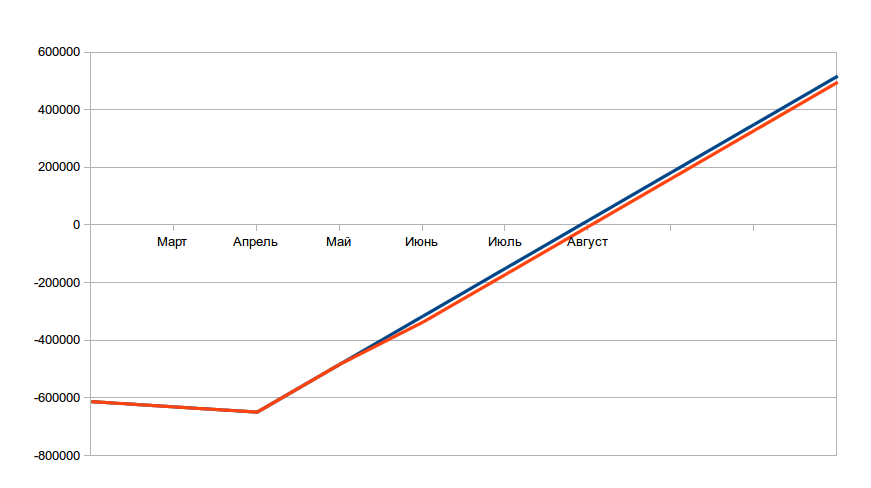
\includegraphics [scale=0.75] {income_complex}
  \caption{Структура дохода, дохода с сервисным обслуживанием} 
  \label{img:income_structure_complex}  
\end{figure}

\vspace{\baselineskip}
\textbf{Себестоимость:} 545871,29  руб.

\textbf{Выручка от продаж за год:}  2400000 руб.

\textbf{Затраты на сервисное обслуживание:} 254862,50 руб.

\textbf{Прибыль от продажи каждого экземпляра ПО:} 32800,10 руб.

\textbf{Вывод:} проект обладает высокими техническими характеристиками и экономически целесообразен.